\section{Gradient Formation}
\begin{frame}
	\frametitle{Gradient Formation}
		\textbf{Objective:} Algorithm to assign unique IDs to Kilobots with respect to a Kilobot using distance as reference.
\end{frame}

\begin{frame}
\frametitle{Flowchart}
\begin{figure}[H]
	\centering
	\fbox{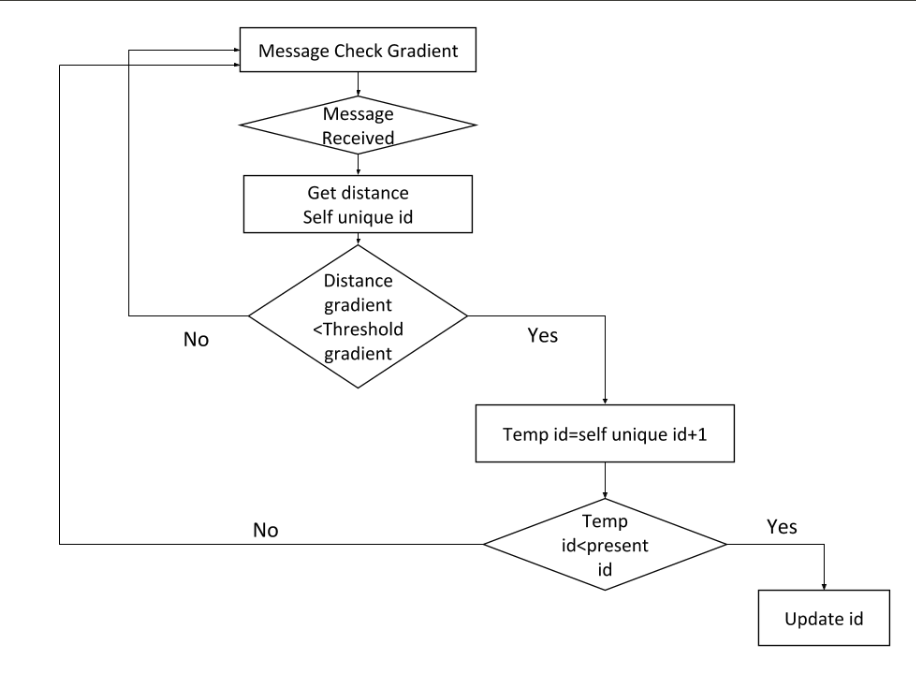
\includegraphics[scale=0.27]{images/flowchart-gradient.png}}
	\caption{Flowchart for gradient formation}
	\label{fig:flowchart-gradient}
\end{figure}
\end{frame}

\begin{frame}
\frametitle{Demonstration}
\begin{figure}[H]
	\centering
	\fbox{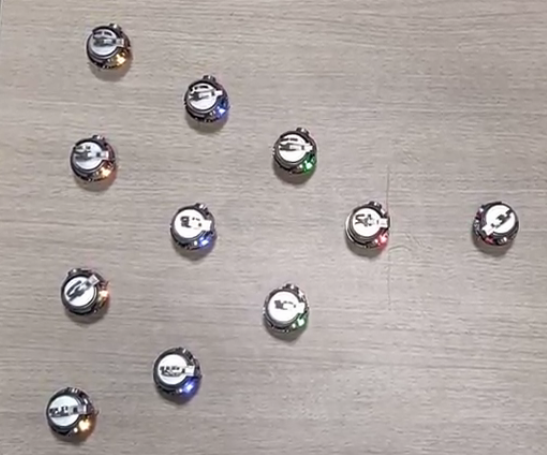
\includegraphics[width=2in]{images/gradient.png}}
	\caption{\href{https://drive.google.com/file/d/1JAcmaJzGgZXJqVzh5EeOXjp7_x3NBJIU/view}{Display of colors as per different ids}}
	\label{fig:gradient-color}
\end{figure}
\end{frame}


